\chapter{REAL-TIME PARTICLE SYSTEMS LIBRARY}

% Introduction
\section{Introduction}
The Real-Time Particle Systems (RTPS) library designed and developed by Ian Johnson\cite{ianPaper}. This library is able to simulate various systems. In our collaboration with Ian Johnson, we created the \texttt{FLOCK} system, which is the system of our concern. RTPS also have a Smooth Particle Hydrodynamics (\texttt{SPH}) system. In this chapter we intend to introduce the RTPS framework and discuss all the extended implementation developed for the \texttt{FLOCK} system. The home folder of RTPS is \texttt{rtpslib}.

\textcolor{red}{*** TODO: Diagram of the RTPS hierarchy ***}
\begin{figure}[htbp]
\begin{center}
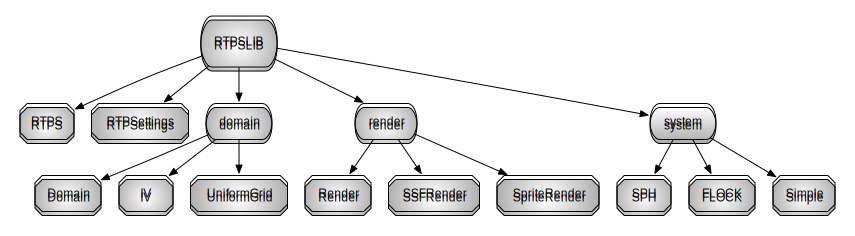
\includegraphics[scale=0.5]{figures/RTPSdiagram.pdf}
\caption{RTPS hierarchy}
\label{RTPSdiagram}
\end{center}
\end{figure}



% RTPS
\section{RTPS}
\texttt{RTPS} is the head class, it is located at \texttt{rtpslib/RTPS.h}. This class creates a particle system given a set of settings\footnote{the settings are going to be discussed in the next section}. \texttt{RTPS} has various instance variables: a \texttt{CL} object which is used to manage the \textit{OpenCL} stuff,  an \texttt{RTPSettings} object to manage the settings of the system and a \texttt{System} object which stores the type of particle system that has been created. Only two methods are defined in this class: \texttt{update()} and \texttt{render()}. Next is the definition of the \texttt{RTPS} constructor used for the \texttt{FLOCK} system.

% RTPS constructor
\begin{cppcode}{0}
RTPS::RTPS(RTPSettings *s, CL* _cli) 
{
	cli = _cli;
 	cl_managed = false;
	settings = s;
	Init();
}
\end{cppcode}

The \texttt{Init()} method would create the respective system\footnote{\texttt{SPH}, \texttt{FLOCK}, or any other defined system} depending on the settings.

% RTPSettings
\section{RTPS Settings}
\texttt{RTPSettings} defines the set of settings for the particle system. The location of this class is at \texttt{rtpslib/RTPSettings.h}. It has the following instance variables defined: the maximum number of particles, the time step, and a \texttt{Domain} object. Also, there is an enumeration variable \texttt{SysType} that defines the names of the three available particle systems. Some of the rendering settings are set and get in this class. Here is the \texttt{RTPSettings} constructor that we use for the \texttt{FLOCK} system.

% RTPSettings constructor
\begin{cppcode}{0}
RTPSettings::RTPSettings(SysType system, int max_particles, float dt, Domain* grid)
{
	changed = false;
	this->system = system;
	this->max_particles = nlpo2(max_particles);
	this->dt = dt;
	this->grid = grid;
}
\end{cppcode}

The parameters for this constructor are the type of system, the maximum number of particles, the time step and the grid domain. The maximum number of particles has to be a power of two that is why \texttt{max\_particles} is process it with the \texttt{nlpo2} function, which takes care of that.

% Domain
\section{Domain}
The class that defines the grid in which the simulation is going to be computed is in \texttt{rtpslib/domain/Domain.h}. This class also stores all the different grid parameters that are needed through out the computation process. The class \texttt{IV} is defined in the \texttt{rtpslib/Domain} folder. This class has the methods which initialize the positions of the particles. Various shapes are defined: rectangles, spheres, and discs. The \texttt{UniformGrid} class is also defined here but not used in the \texttt{FLOCK} system.

% Render
\section{Render}
Most of the render code developed in for the RTPS library has been developed by Andrew Young. The \texttt{rtpslib/render/Render.h} class takes care of rendering the particles. The \texttt{RTPSettings} class has an enumeration that defines the available types of rendering defined in the \texttt{Render} class: Render (Points), Sprites, and Screen Space. For our system \texttt{FLOCK}, we only use the \textit{Points} render and the \texttt{Sprites} render. A special shader was defined in order to use Sprites, \texttt{rtpslib/render/shaders/boid\_tex\_frag.glsl}. With this shader we are able to render any image with transparent background as a boid.

% System
\section{System}
\texttt{System} is the class that is inherited by the particular systems defined in the \texttt{RTPSettings} system type enumeration. The location of this class is \texttt{rtpslib/system/System.h}. It contains virtual functions that are shared by the systems. These functions are related to the \texttt{Render} object,  the \texttt{Domain} objects, the \texttt{Hose} object, and the VBO objects.

% Common
\subsection{Common}
Inside the \texttt{rtpslib/system/common} folder are the files that are shared by the systems. These files are used to compute the nearest neighbors of each boid. The approach taken is the following:

\textcolor{red}{*** TODO:  list the steps for the neighbor search ***}

Also, the definition of the \texttt{Hose} class is share. Hoses are very useful for doing demonstrations. In the \texttt{rtpslib/system/common/cl\_src} folder are the \textit{OpenCL} implementation of the respective kernels.

% SPH
\subsection{SPH}
The \texttt{SPH} system is the main system of the RTPS library. It was developed and it is currently maintained by Ian Johnson\cite{ianBlog}\cite{ianPaper}. This system simulate uses the SPH formulation to compute the different forces between particles, for more detailed information please refer to Ian Johnson Master Thesis\cite{ianThesis}.

% FLOCK
\subsection{FLOCK}
\texttt{FLOCK} system is the system of our concern. We used the \texttt{SPH} system as a guide to create the \texttt{FLOCK} system. Both of these systems are inherited from the \texttt{System} class. \texttt{FLOCK} has a main class located at \texttt{rtpslib/system/FLOCK.h}. Also, we developed a class for the settings called \texttt{FLOCKSettings.h}, and the different implementation for the flocking behavior which can be found at the \texttt{rtpslib/system/flock} folder. Figure \label{flockdiagram} shows the hierarchy of the \texttt{FLOCK} system.

\textcolor{red}{*** TODO: Diagram of the FLOCK hierarchy ***}

Next, we are going to discuss in detail the implementation of the classes shown in the diagram of Figure \label{flockdiagram}.

% FLOCK class
\subsubsection{FLOCK class}
The \texttt{FLOCK} class is the main class of our system. The location of the class is at \texttt{rtpslib/system/FLOCK.h}. In the header file we defined the prototypes of the functions to that are used to insert particles to our system. Also, all the vectors used to store the information of our system are declared in here. These vectors stores the data that is going to be handle in the CPU and in the GPU.

The implementation starts at the \texttt{FLOCK.cpp}. This is the code used in the constructor of  our system.

\begin{cppcode}{0}
FLOCK::FLOCK(RTPS *psfr, int n)
 {
 	//store the particle system framework
 	ps = psfr;
	settings = ps->settings;
	grid = settings->grid;
	max_num = n;
	
	// initial number of particles
	num = 0;
 
 	//seed random
 	srand(time(NULL));
 
 	// get the path 
	resource_path = ps->settings->GetSettingAs<std::string>("rtps_path");

	// create a buffer for the parameters in the GPU
	std::vector<FLOCKParameters> vparams(0);
	vparams.push_back(flock_params);
	cl_FLOCKParameters= Buffer<FLOCKParameters>(ps->cli, vparams);
 
 	// calculate and update the parameters
	calculate();
	updateFLOCKP();

	// get the spacing
	spacing = settings->GetSettingAs<float>("Spacing");
	
	//set up the grid
	setupDomain();
	
	// set up the timers
	setupTimers();
	
	//setup the sorted and unsorted arrays
	prepareSorted();
 	 
#ifdef CPU
	printf("RUNNING ON THE CPU\n");
#endif
#ifdef GPU
	printf("RUNNING ON THE GPU\n");
	
	// create the directories in which the kernels are going to be copied
	flock_source_dir = resource_path + "/" + std::string(FLOCK_CL_SOURCE_DIR);
	common_source_dir = resource_path + "/" + std::string(COMMON_CL_SOURCE_DIR);
	
	// include the directories
	ps->cli->addIncludeDir(flock_source_dir);
	ps->cli->addIncludeDir(common_source_dir);
	
	// initialize our objects, these objects would take care of the simulation
	hash = Hash(common_source_dir, ps->cli, timers["hash_gpu"]);
	bitonic = Bitonic<unsigned int>(common_source_dir, ps->cli );
	cellindices = CellIndices(common_source_dir, ps->cli, timers["ci_gpu"] );
	permute = Permute(common_source_dir, ps->cli, timers["perm_gpu"] );
	rules = Rules(flock_source_dir, ps->cli, timers["rules_gpu"]);
	euler_integration = EulerIntegration(flock_source_dir,ps->cli,timers["euler_gpu"]);
		
	// create the renderer object depending on the render type		
	setRenderer(); 
}
\end{cppcode}

Let us discuss what we are doing in the constructor. First, we copy the particle system \texttt{psfr} to our instance variable \texttt{ps}. We do the same for the settings, the grid, and the maximum number of particles. The actual number of particles is set to zero. Then, we initialize the seed to generate random numbers. Next, we get the path of where we compiled the program. A buffer is then created to store the parameters in the GPU. Then, the initial \texttt{FLOCKParameters} are calculated and updated. The calculation means to set parameters to the default values, then when they are updated if the user changed any of them only those parameters are going to change in value. Then, we get the spacing that is used between the particles. Then, the domain and the timers are set up. For the domain we basically initialize the grid parameters and for the timers we allocate memory of each of the timers that we are going to use.

The next step is to call \texttt{prepareSorted()}. What \texttt{prepareSorted()} does is to initialize the different vectors we created i.e \texttt{velocities}, \texttt{flockmates}, etc. It also create the VBOs and copy the positions and color vectors to the respective VBOs\footnote{VBOs are used to store data with rendering purposes}. Then, if we are using the GPU we initialize the different \texttt{Buffer} objects with the respective CPU arrays and copy the parameters to the GPU. After \texttt{prepareSorted()} is done, if we are using the CPU we are done initializing our system, otherwise we still need to a few more stuff. A final OpenCL setup related with the directories in which the kernels are going to be copied is done. Then, the different objects used for the neighbor search and the flocking simulation are created. Finally, the \texttt{setRenderer()} function is called, and it creates the \texttt{renderer} object depending on which render type we set in the \texttt{RTPSettings}.

A very important function in this file is the \texttt{update()} function. This function is in charge of doing the calls of the functions that are going to update the positions of the boids at each time step. If we were using only the CPU, we would call \texttt{updateCPU()} which only calls the function \texttt{cpuRules()}, then the rules are computed sequentially. We developed the CPU code for testing purposes only, and to do benchmarks. On the other hand, if we were using the GPU to do the calculations, we would call \texttt{updateGPU()} which calls the OpenCL kernels to do the neighbor search and then to compute the flocking rules. We would discuss these kernels in more detail in the \textbf{Rules class} subsection.

\textit{How do we insert particles into the system?} There are a few functions defined \texttt{addBox} , \texttt{addBall}, and \texttt{addHose}, that insert particles to the system. These functions first, initialize the positions of the particles using the functions defined in \texttt{IV.h} class, then the positions are send it to the GPU. This ended up the description of the \texttt{FLOCK} class.
 
% FLOCKSettings class
\subsubsection{FLOCKSettings class}
In order to run a simulation we need some settings, the flocking specific settings are in the class \texttt{rtpslib/system/FLOCKSettings.h}. The \texttt{FLOCKParameters} struct is defined in here. Some of the parameters in this struct are: the simulation scale, the searching radius, the maximum speed of the boids, the weights of each of the rules, and a few others. In the \texttt{FLOCKSettings.cpp} are defined the functions \texttt{calculate()} and \texttt{updateFLOCKP()} which are called in the constructor of \texttt{FLOCK}, and we mentioned above that they initialize and update the parameters.

% Rules class
\subsubsection{Rules class}

% Euler Integration class
\subsubsection{EulerIntegration class}

